\section{MOS Diode}
\subsection{Gegenüberstellung Diodentypen}

%NOTE: Platzhalter! -> wird mit überarbeitetem pdf ersetzt
%TODO: [Simi]: pdf

\begin{tabularx}{\columnwidth}{@{}c c c c@{}}
    Ideale Diode ($V_F = V_{F0}$) & Reale Diode & \multicolumn{2}{c}{MOS-Diode}\\
    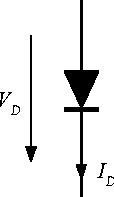
\includegraphics[height=1.75cm]{images/diode_ideal_symbol.pdf} & 
    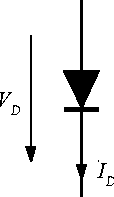
\includegraphics[height=1.75cm]{images/diode_real_symbol.pdf} & 
    \parbox[t]{\widthof{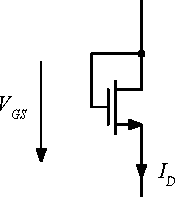
\includegraphics[height=1.75cm]{images/diode_nmos_symbol.pdf}}}{%
        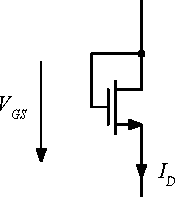
\includegraphics[height=1.75cm]{images/diode_nmos_symbol.pdf}\\
        \phantom{------} NMOS} & % this \phantom{------} is a bit of a hacky way to get the text to where it should be... maybe we'll change it later on
    \parbox[t]{\widthof{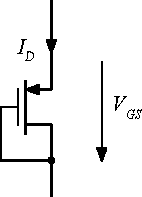
\includegraphics[height=1.75cm]{images/diode_pmos_symbol.pdf}}}{%
        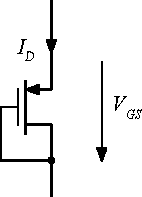
\includegraphics[height=1.75cm]{images/diode_pmos_symbol.pdf}\\
        PMOS} \\
    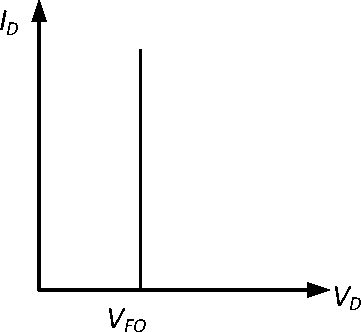
\includegraphics[width=.3\columnwidth]{images/diode_ideal_kennlinie.pdf} & 
    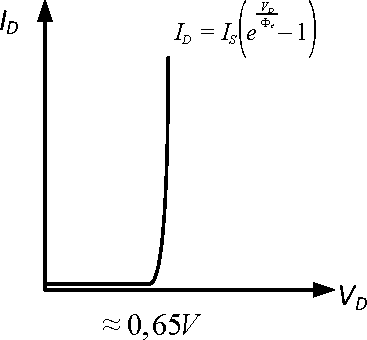
\includegraphics[width=.3\columnwidth]{images/diode_real_kennlinie.pdf} & 
    \multicolumn{2}{c}{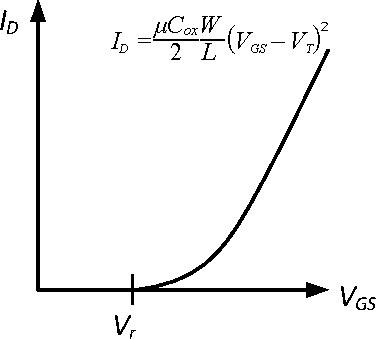
\includegraphics[width=.3\columnwidth]{images/diode_mos_kennlinie.pdf}} \\ 
\end{tabularx}


\subsection{Arbeitsbereich der MOS Diode}

Die MOS Diode arbeitet \textbf{(in strong inversion) immer in Sättigung}, da die Sättigungsbedingung aufgrund der Verbindung der Gate- und Source-Anschlüsse immer erfüllt ist:
\[
    V_\text{DS} = V_\text{GS} > V_\text{GS} - V_\text{T}
\]
\textbf{Hinweis:} Die Forwardspannung bestimmt, ob die MOS Diode in strong- oder weak inversion betrieben wird.
\textbf{Der 'Normalfall' ist strong inversion.}


\subsection{Arbeitspunkteinstellung}

\subsubsection{Arbeitspunkteinstellung mittels Drainstrom}

\begin{minipage}[t]{0.3\columnwidth}
    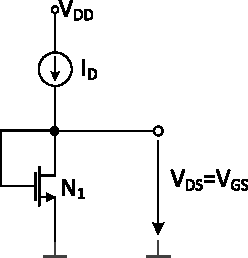
\includegraphics[width=\columnwidth, align=t]{images/04_MOS_diode_mit_stromquelle.pdf}
\end{minipage}
\hfill
\begin{minipage}[t]{0.66\columnwidth}
    Aus der Drainstrom-Gleichung (strong inversion, Sättigung) lässt sich die Spannung über der Diode als Funktion des Eingangsstroms berechnen:
    \[
        V_\text{DS} = V_\text{GS} = V_T + \sqrt{\frac{2 I_\text{D}}{\mu C_\text{ox} \frac{W}{L}}}
    \]

    %CHECK: [Simi] @ Flurin: WO kommt das her? Ist das relevant?   
    \[
        V_{GS} = V_\text{M} + n_M V_\text{temp} \ln{\frac{I_\text{D}}{I_m' \frac{W}{L}}}
    \]
\end{minipage}


\subsubsection{Arbeitspunkteinstellung mittels Seriewiderstand}

\begin{minipage}[t]{0.3\columnwidth}
    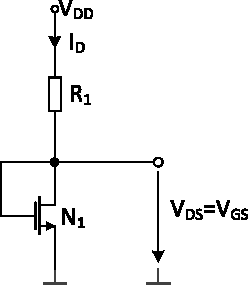
\includegraphics[width=\columnwidth, align=t]{images/04_MOS_diode_mit_widerstand.pdf}
\end{minipage}
\hfill
\begin{minipage}[t]{0.66\columnwidth}
    Der Arbeitspunkt kann auf zwei Arten ermittelt werden:

    \smallskip
    
    \begin{outline}
        \1 Grafisch durch Einzeichnen der Lastgerade des Drainwiderstands $R_1$ in der Kennlinie $I_D = f(V_{\rm GS})$
            \2 Leerlaufspannung: $V_{\rm GS,0} = V_{\rm DD}$
            \2 Kurzschluss-Strom: $I_{D, 0} = \frac{V_{\rm DD}}{R_1}$ \\
            \textrightarrow\ Schnittpunkt entspricht Arbeitspunkt
            \smallskip
        \1 Rechnerisch mittels folgender Formel
        $$ I_D = \frac{V_{\rm DD} - V_{\rm GS}}{R_1} = \frac{\mu C_{\rm OX}}{2} \frac{W}{L} (V_{\rm GS} - V_T)^2 $$
    \end{outline}
\end{minipage}


\subsection{Kleinsignalersatzschaltung}

\begin{minipage}[t]{0.3\columnwidth}
    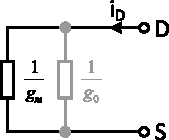
\includegraphics[width=\columnwidth, align=t]{images/04_MOS_diode_ersatzschaltung_vereinfacht.pdf}
\end{minipage}
\hfill
\begin{minipage}[t]{0.65\columnwidth}
    Die Kleinsignalersatzschaltung kann (leicht angepasst) vom MOS Transistor übernommen werden.
    \begin{align*}
        \text{Allgemein:} \quad             r_\text{\rm MD}  &= \frac{1}{g_m + g_0} = \frac{1}{g_m} \parallel r_{DS} \\
        \text{\textbf{Praxis:}} \quad       r_\text{\rm MD} &\approx \frac{1}{g_m} = \frac{1}{\sqrt{2 \mu C_\text{ox} \frac{W}{L} I_\text{D}}}
    \end{align*}

\end{minipage}


\subsection{Anwendungen}

\subsubsection{Spannungsreferenz}
\label{Spannungsreferenz}

\begin{minipage}[t]{0.44\columnwidth}
    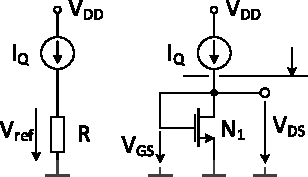
\includegraphics[width=\columnwidth, align=t]{images/04_MOS_diode_spannungsreferenz.pdf}
\end{minipage}
\hfill
\begin{minipage}[t]{0.52\columnwidth}
    \textbf{Voraussetzung: } Referenzstrom $I_Q$
    \smallskip

    \begin{itemize}
        \item[+] Kleinerer Flächenanspruch als Widerstand
        \item[+] Eingangsspannung wird durch relativ tiefen $\Delta r_{\rm MD}$ geglättet
        \item[-] Genauer als mit Widerstand, jedoch noch immer eher ungenau
        \item[-] $r_{\rm MD}$ kann nur schlecht verändert werden
    \end{itemize}
\end{minipage}


\subsubsection{Spannungsstabilisator}

\begin{minipage}[t]{0.48\columnwidth}
    \begin{outline}
        \1 MOS-Dioden Schaltung aus Abschnitt \ref{Spannungsreferenz} mit Widerstand statt Stromquelle
        \1 AC-Störung wird oberhalb von $R$ eingespeist (gegenüber GND)
    \end{outline}
\end{minipage}
\hfill
\begin{minipage}[t]{0.48\columnwidth}
    \raggedright
    
    \begin{outline}
        \1 Kleinsignalersatzschaltung des beschriebenen Aufbaus:
            \2 Spannungsteiler aus $R$ (gross) und $r_{\rm MD}$ (klein) \\
            \textrightarrow\ AC-Störspannung $v_0$ am Ausgang ($V_{\rm DS} + v_0$) sehr klein
    \end{outline}
\end{minipage}



\subsubsection{Spannungsteiler}

Spannungsteiler könnten auf mehrere Arten realisiert werden. \textrightarrow\ \textbf{Variante (b) am Besten!}

\vspace{-0.2cm}

\begin{ctabular}{@{}c cc cc cc@{}}
    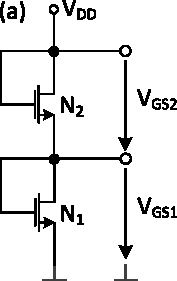
\includegraphics[height=3cm, align=t]{images/04_MOS_diode_spannungsteiler_a.pdf}    & &
    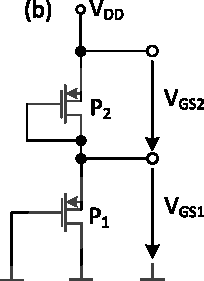
\includegraphics[height=3cm, align=t]{images/04_MOS_diode_spannungsteiler_b.pdf}    & & 
    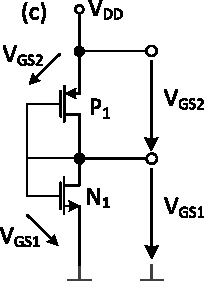
\includegraphics[height=3cm, align=t]{images/04_MOS_diode_spannungsteiler_c.pdf}    & &
    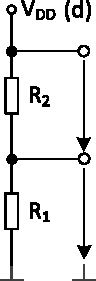
\includegraphics[height=3cm, align=t]{images/04_MOS_diode_spannungsteiler_d.pdf}    \\
\end{ctabular}


\begin{minipage}[t]{0.36\columnwidth}
    Schaltung (a)
    \begin{itemize}
        \item[+] Gleiche Elemente (nMOS)
        \item[-] Body-Effekt bei $N_2$
    \end{itemize}
   
    \smallskip

    \textbf{Schaltung (b)}
    \begin{itemize}
        \item[+] Gleiche Elemente (pMOS) \\
            \textrightarrow\ gutes Matching
        \item[+] Kein Body-Effekt (pMOS)
    \end{itemize}
\end{minipage}
\hfill
\begin{minipage}[t]{0.6\columnwidth}
    Schaltung (c)
    \begin{itemize}
        \item[+] Kein Body-Effekt
        \item[-] Komplementäre Elemente
            \textrightarrow\ schlechtes Matching
    \end{itemize}
   
    \smallskip

    Schaltung (d)
    \begin{itemize}
        \item[+] Gute \textbf{relative} Genauigkeit
        \item[-] Schlechte \textbf{absolute} Genauigkeit
        \item[-] Braucht viel Platz 
    \end{itemize}
\end{minipage}

\smallskip

\begin{minipage}[c]{0.55\columnwidth}
    Weil für die Ströme gilt, dass $I_{D1} = I_{D2}$ ergibt sich das das Spannungsverhältnis
\end{minipage}
\hfill
\begin{minipage}[c]{0.4\columnwidth}
    \[
        \frac{\abs{V_{\rm GS1} - V_{\rm T1}}}{\abs{V_{\rm GS2} - V_{\rm T2}}} = \sqrt{\frac{(W / L)_2}{(W / L)_1}}
    \]
\end{minipage}



